% Sovereign Integrity Protocol License v1.1; see the repository LICENSE.
\documentclass[11pt]{article}
\usepackage[T1]{fontenc}
\usepackage[margin=1in]{geometry}
\usepackage{amsmath,amssymb,amsthm,booktabs,graphicx}
\usepackage[expansion=false]{microtype}
\usepackage[hidelinks]{hyperref}
\newtheorem{proposition}{Proposition}
\newcommand{\Tr}{\operatorname{Tr}}
\newcommand{\Rea}{\operatorname{Re}}
\newcommand{\Ima}{\operatorname{Im}}
\title{Complete Scalar Actions and Identifiability Boundaries\\in the ACS Framework}
\author{Brad Wallace\\\small Independent Researcher}
\date{24 September 2026}
% Publication typography: portable paths, bounded tables, paragraph flexibility.
\usepackage{xurl,adjustbox}
\setlength{\emergencystretch}{3em}
\begin{document}
\maketitle
\begin{abstract}
We consolidate the action-to-spectrum audit of the specified minimal
Pati--Salam scalar sector of the Asymmetric Codependent Systems framework.
The calculation retains 68 real scalar coordinates, 17 real quartic
coefficients, four quadratic coefficients and the trace kinetic metric.
Six quartic directions are invisible on the neutral background family.
Explicit bounded potentials with identical neutral data nevertheless have
different transverse stability, and the usual two-trace restriction is not
generically closed under one-loop running. A homogeneous family of complete
actions changes all physical masses without changing dimensionless labels;
the result extends to arbitrary complex flavor matrices and the stated
one-loop potential. Independent finite-running calculations retain boundary
sensitivity. These results establish a usable forward calculation and precise
limits on what it identifies. They do not select a physical vacuum, a unique
mass scale or measured flavor data. Exact identities, numerical qualifications,
source errors and unresolved physical inputs are reported separately.
\end{abstract}

\section{Introduction}
An algebraic representation specifies allowed interactions and charge labels.
A physical prediction also requires normalized coefficients, a vacuum and a
prescription relating the model to measured quantities. The purpose of this
paper is to determine which of these steps follow from the supplied ACS
action and which remain additional data. It is a consolidation and correction
of the repository's calculations, not a claim that an unrestricted theory of
matter has been completed.

Our organization follows conventional scalar-potential and matching studies:
define the fields and conventions, analyze the full potential, distinguish
local stability from boundedness and global selection, and state the domain
of the matching calculation. Orbit-space restrictions are relevant to
boundedness questions~\cite{Kannike}. Finite matching also requires attention
to mixed heavy/light contributions and normalization~\cite{Jiang,Gherardi}.
These references provide methods and context, not evidence for an ACS
parameter-selection law.

\section{Fields, action and normalization}
The gauge group is
$SU(4)\times SU(2)_L\times SU(2)_R$, with
$\Phi\sim(1,2,2)$ and $\Delta\sim(\overline{10},1,3)$.
We represent $\Phi$ by a complex $2\times2$ matrix and $\Delta$ by three
complex symmetric $4\times4$ matrices $D_a$. Thus $\Phi$ supplies eight
and $\Delta$ supplies sixty real coordinates. Define
\begin{equation}
 N_\Phi=\Tr\Phi^\dagger\Phi,\qquad d_\Phi=\det\Phi,
 \qquad N_\Delta=\sum_{a=1}^3\Tr D_a^\dagger D_a.
\end{equation}
The potential in the inherited invariant basis is
\begin{equation}\label{eq:potential}
 V(x)=\Omega+\sum_{i=1}^4m_i I_{2i}(x)
             +\sum_{j=0}^{16}\lambda_j I_{4j}(x),
\end{equation}
where $m_i$ is a mass-squared coefficient, not a mass. The quadratic basis is
$(N_\Phi,\Rea d_\Phi,\Ima d_\Phi,N_\Delta)$.
The real quartic basis is summarized in Table~\ref{tab:basis}.

\begin{table}[ht]
\centering\small
\begin{adjustbox}{max width=\linewidth}\begin{tabular}{cl}
\toprule
Indices & Invariants, in the archived normalization\\
\midrule
$0$--$5$ & $N_\Phi^2, |d_\Phi|^2,\Rea d_\Phi^2,\Ima d_\Phi^2,
 N_\Phi\Rea d_\Phi,N_\Phi\Ima d_\Phi$\\
$6$--$10$ & $\|P_{35,0}(D\otimes D)\|^2,\|P_{35,2}(D\otimes D)\|^2,
 \|P_{20,0}(D\otimes D)\|^2,$\\
 & $\|P_{20,2}(D\otimes D)\|^2,\|P_{45,1}(D\otimes D)\|^2$\\
$11$--$12$ & $\Rea H_\Delta,\Ima H_\Delta$\\
$13$--$16$ & $N_\Phi N_\Delta,\Rea d_\Phi N_\Delta,
 \Ima d_\Phi N_\Delta,J_\Phi\cdot J_\Delta$\\
\bottomrule
\end{tabular}\end{adjustbox}
\caption{The first projector label denotes the color-representation
dimension and the second the weak spin. The five norms sum to
$N_\Delta^2$. The phase-sensitive invariant $H_\Delta$ and the weak-vector
contraction use the exact component definitions in the supplied basis code;
their coefficients cannot be compared across normalizations without that map.}
\label{tab:basis}
\end{table}

The trace kinetic terms give
$\mathcal L_{\rm kin}=\tfrac12\partial_\mu x^TG\partial^\mu x$,
with $G=2$ on $\Phi$ and diagonal $D_a$ entries and $G=4$ on off-diagonal
$D_a$ entries. If $H$ is the raw real-coordinate Hessian, masses solve
\begin{equation}
 Hv=m^2Gv,\qquad H_c=G^{-1/2}HG^{-1/2}.
\end{equation}
A raw Hessian eigenvalue is consequently not automatically a physical mass.
For one radial coordinate with kinetic coefficient $Z$ and potential
$c_4r^4$, the convention $h=\sqrt Zr$ gives
\begin{equation}
 V=\frac{\lambda_{\rm can}}4h^4,
 \qquad \lambda_{\rm can}=\frac{4c_4}{Z^2}.
\end{equation}
Consistent changes of field coordinates leave this ratio unchanged.
Multiplying the entire action by an unspecified constant $C$ instead changes
the canonically normalized quartic to $\lambda_{\rm can}/C$.

\section{What a neutral restriction cannot determine}
Consider
\begin{equation}\label{eq:neutral}
 \Phi=\operatorname{diag}(a,b e^{i\alpha}),\qquad
 (D_1,D_2,D_3)=\frac{dE_{44}}{\sqrt2}(1,-i,0).
\end{equation}
For nonzero unequal $a,b$ and nonzero $d$, the unbroken group is
$SU(3)_c\times U(1)_{\rm em}$. The 21 gauge generators have twelve
independent orbit directions, leaving 56 physical real scalar directions.
The entire neutral restriction has quartic rank eleven. The missing six
directions are $I_6,I_8,I_9,I_{10},\Rea H_\Delta,\Ima H_\Delta$.
The first four affect transverse masses. At the rank-one color background,
$H_\Delta$ has zero value, gradient and Hessian but nonzero cubic vertices.
For example, a specified diagonal perturbation gives
$H_\Delta=3ABCd/\sqrt2$ in the archived normalization.

\subsection{An explicit stability counterfamily}
Take the bounded family
\begin{align}
 V_4={}&N_\Phi^2+|d_\Phi|^2+N_\Delta^2
 +k(I_6+I_8+I_9+I_{10})\nonumber\\
 &+\frac{\Rea H_\Delta}{100}+\frac{\Ima H_\Delta}{50}
 +\frac{N_\Phi N_\Delta}{10}+\frac{J_\Phi\cdot J_\Delta}{50},\\
 V_2={}&-\frac{2743}{7200}N_\Phi
 -\frac{41}{240}\Rea d_\Phi-\frac{1259}{625}N_\Delta.
\end{align}
The background $a=1/3,b=1/5,d=1,\alpha=0$ is stationary for each
tested $k$. The neutral potential and its four physical neutral masses
are identical, while Table~\ref{tab:stability} shows different full spectra.
The boundedness certificate and exact sparse-polynomial calculation are
retained in the canonical-vacuum evidence package. This is a deliberately
chosen witness family, not an observed particle fit.

\begin{table}[ht]
\centering
\begin{adjustbox}{max width=\linewidth}\begin{tabular}{rrrr}
\toprule
$k$ & Positive physical modes & Flat physical modes & Negative physical modes\\
\midrule
$1/5$ & 56 & 0 & 0\\
$0$ & 44 & 12 & 0\\
$-1/5$ & 6 & 0 & 50\\
\bottomrule
\end{tabular}\end{adjustbox}
\caption{Twelve gauge Goldstone directions are excluded from every row.
The neutral data alone do not distinguish the rows.}
\label{tab:stability}
\end{table}

There is an exact independent negative-direction witness. The canonically
normalized real part of $D_{3,00}$ has
\begin{equation}
 m^2=\frac53k+\frac4{5625}.
\end{equation}
It is negative at $k=-1/5$. At $k=1/5$, the minimum physical scalar
mass-squared is approximately $0.04321111$. Positivity of this local spectrum
does not prove that the point is the global minimum or that quantum decay is
absent.

\section{Radiative closure and matching}
Let $B=32\pi^2d/d\log\mu$. The additive gauge source for the five
Hermitian $\Delta$ quartics is
\begin{equation}
 B\begin{pmatrix}\lambda_6\\\lambda_7\\\lambda_8\\\lambda_9\\\lambda_{10}\end{pmatrix}_{\!g}
 =g_4^4\begin{pmatrix}45\\45\\9\\9\\-3\end{pmatrix}
 +g_4^2g_R^2\begin{pmatrix}-72\\36\\72\\-36\\12\end{pmatrix}
 +g_R^4\begin{pmatrix}36\\18\\36\\18\\6\end{pmatrix}.
\end{equation}
These terms were checked monomial by monomial against the complete gauge
Gram, with scalar and Yukawa contributions treated separately. The radial
source, gauge sources and a further scalar-loop contraction require the
full five-dimensional Hermitian space for generic independent gauge couplings.
This does not preclude a future derived relation among boundary values.

The two holomorphic coefficients satisfy, at this order,
\begin{equation}
 B\lambda_j=\left[\frac{80}{3}\lambda_8+\frac{64}{3}\lambda_9
 -108g_4^2-48g_R^2+8\Tr(F^\dagger F)\right]\lambda_j,
 \quad j=11,12.
\end{equation}
Their simultaneous zero surface is thus preserved by these one-loop
equations. It is a boundary choice, and the associated classical global
charge has weak mixed anomalies. A perturbative zero surface is not a proof
of exact quantum charge protection.

For illustration, both natural readings of the historical two-trace
$\Delta$ potential require $\lambda_6=\lambda_7$. At the source point
$\rho_1=8/9,\rho_2=0$, equal gauge couplings $4/3$ and zero Yukawas,
the complete equations give
$B(\lambda_6-\lambda_7)=-2560/9$.
The reduced ansatz therefore fails a direct closure test.

Tree elimination is meaningful after an action and branch are specified.
For a radial deviation $y$ with terms $\lambda_7y^2+KXy$, eliminating
$y$ gives the correction $-K^2X^2/(4\lambda_7)$.
The retained finite one-loop study additionally includes mixed heavy/light
effects, infrared subtraction and finite kinetic normalization on its
declared stable branch. It was checked against 80-digit limits. It assumes
a particular light doublet, portal structure and real diagonal flavor;
general noncommuting-flavor, mixed-quartic finite matching is not asserted.

\section{A complete-action scale family}
\begin{proposition}\label{prop:scale}
For the flat-space action with potential~\eqref{eq:potential}, fix the
dimensionless coefficients and positive kinetic metric. Simultaneously replace
\begin{equation}
 x\mapsto ax,\quad m_i\mapsto a^2m_i,\quad
 \Omega\mapsto a^4\Omega,\quad\mu\mapsto a\mu,
 \qquad a>0.
\end{equation}
Stationary configurations map to stationary configurations, physical
mass-squared eigenvalues scale by $a^2$, and their signs and ratios are
unchanged. The same scaling holds for gauge masses and fermion squared
singular masses, including complex noncommuting Yukawa matrices.
\end{proposition}
\begin{proof}
Each $I_2$ is homogeneous of degree two and each $I_4$ of degree four.
Consequently $V,\nabla V,H$ scale by $a^4,a^3,a^2$, respectively. Since
$G$ is fixed, the canonical Hessian has the same scaling. Infinitesimal
gauge-orbit vectors are linear in $x$, so their mass Gram is quadratic.
The Weyl mass matrix is linear in the scalar background at fixed Yukawas;
its singular values scale by $a$. No diagonal-flavor assumption enters.
\end{proof}

The statement compares physically different actions. It is not a coordinate
symmetry of one fixed action. At a qualified stable background the one-loop
potential has the form
\begin{equation}
 V_1=\frac1{64\pi^2}\sum_\nu n_\nu M_\nu^4
 \left(\log\frac{M_\nu^2}{\mu^2}-c_\nu\right).
\end{equation}
The logarithms are unchanged under the simultaneous transformation, so
$V_1$ scales by $a^4$. Two component tests use all 68 scalars, 21 gauge
directions and a complex 48-Weyl example; normalized residuals are below
$10^{-10}$ for the component scaling and $10^{-9}$ for the one-loop sum.
These checks support the exact homogeneity argument; they do not promote
the one-loop approximation to an all-orders result.

A fixed measured Newton constant could provide extra dimensional data, but
the matter-sector matching relation would still have to be derived.
Dimensional transmutation also retains an integration constant:
$\Lambda=\mu\exp[-1/(2bg^2(\mu))]$ for the stated one-loop equation.
The beta function alone does not select $\Lambda$ in physical units.

\section{Running does not supply the missing selector}
A finite regular flow of a smooth ordinary differential equation is locally
invertible. Focusing may reduce sensitivity without making all boundary
data identical. The historical source's one-loop SM truncation gives the
three conditional pairs
\begin{equation}
 (\lambda_{\rm UV},\lambda_{\rm IR})\simeq
 (0.08,0.1685520),\ (0.1283001,0.1806315),\ (0.18,0.1898121).
\end{equation}
A variational equation and independent boundary differences agree on
$d\lambda_{\rm IR}/d\lambda_{\rm UV}=0.2088898$ at the middle point.
The comparison input is $0.1294$. The middle RG output corresponds to
an approximately $148$ GeV tree mass proxy, not a pole-mass prediction. Mixed historical input conventions
and omitted thresholds preclude a precision phenomenological interpretation.

The source's fixed-gauge four-quartic proxy can also be resolved exactly.
Write $\lambda_i=(16/9)(x,y,z,w)_i$. Its fourth equation is
$4w(x+y-3)=0$. If $w\ne0$, the second equation becomes
$2z^2+2w^2+3=0$, which has no real solution. With $w=0$, the third
equation splits into $z=0$ or $z=(3-x-y)/2$. Exact elimination and
Sturm root counts leave precisely two real solutions:
\begin{equation}
 (\lambda_1,\lambda_2,\lambda_3,\lambda_4)\simeq
 (0.1811535,0.5106919,0,0),\quad(0.6447133,0.5764245,0,0).
\end{equation}
Neither gives $2\sqrt3/27$. These are roots of a fixed-gauge proxy, not
fixed points of the complete running action. The full archived program
timed out in its symbolic solve; that execution failure remains recorded.
The independent real-root result does not relabel the failed replay.

\begin{figure}[ht]
\centering
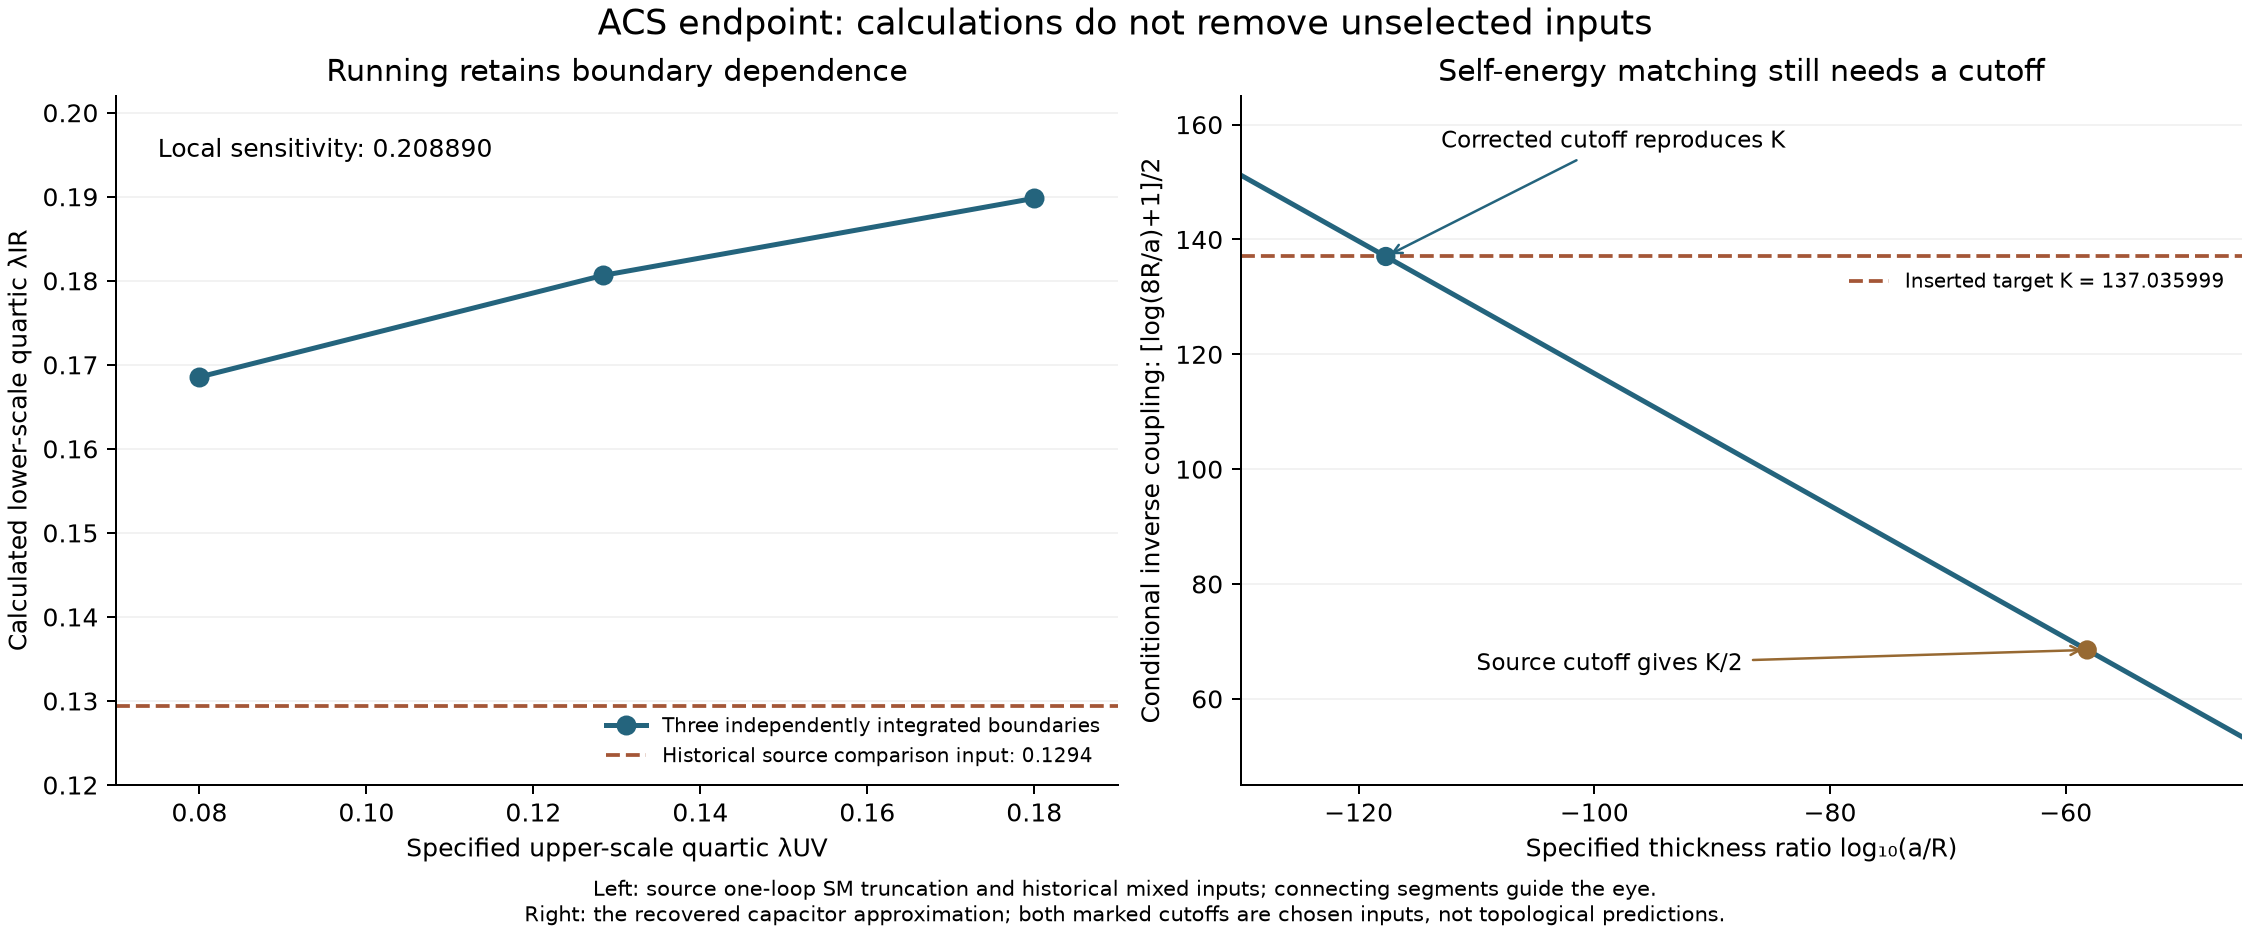
\includegraphics[width=\textwidth]{../../docs/condensate_energy/endpoint_audit/endpoint-boundary.png}
\caption{Left: explicit residual sensitivity to a chosen UV boundary.
Right: the separate capacitor proposal, discussed in the companion carrier
paper, reproduces a target only after a cutoff is specified. Both panels are
conditional calculations, not empirical parameter predictions.}
\end{figure}

\section{Discussion and conclusions}
The completed forward calculation is useful precisely because it exposes
what the neutral restriction misses. It supplies physical spectra in a
specified kinetic metric, tests symmetry and radiative closure, and supports
conditional matching calculations. It also supplies explicit countermodels
to uniqueness claims. A numerical minimizer cannot choose which allowed
action nature uses, and a source expression matched to an inserted value
does not derive that value.

The remaining physical requirements are a normalized microscopic
condensate-to-field map, a coefficient and flavor selection law, and a
physical vacuum and matching prescription. The present result is
underdetermination within the reviewed assumptions, not a no-go theorem
against a future model that adds justified premises. It neither proves RH
nor identifies a universal physical origin for prime or zero statistics.

\appendix
\section{Evidence and reproduction}
The computational record is in \texttt{docs/condensate\_energy/}, with
the canonical, hidden-coupling, action-matching, finite-matching and endpoint
subdirectories separating claims and approximations. Source snapshots,
failed runs, exact polynomials and independent numerical qualifications
are retained. The publication driver in
\nolinkurl{scripts/verify_publication.py} checks the portable evidence
integrity and invokes the declared scientific checks; archive recovery
programs requiring the original local drives are not advertised as portable.
Checks are not independent experiments. The endpoint's 95 passing checks
and one incomplete source replay have different meanings and remain separate.

\section*{Author Statement, Neurodiversity Context, and Methodological Note on Assistive Tooling}
\noindent\textbf{Independent Research and Author Genesis.} 
All original hypotheses, physical models, and mathematical architectures in this paper and across the ACS Framework are the independent intellectual creation of the human author, Bradley Wallace, representing an estimated 5,000--6,000 hours of intensive solo research.

\vspace{0.5em}
\noindent\textbf{Neurodiversity Accommodation and Analog MoE Assistive Tooling.}
The author navigates dyslexia and ADHD. To bridge the friction associated with conventional reading and written composition, the author designed and operated a human-in-the-loop ``Analog Mixture-of-Experts'' (MoE) workflow utilizing an ensemble of AI systems: OpenAI GPT, Anthropic Claude, xAI Grok, DeepSeek, Google Gemini, Cursor, and Google DeepMind Antigravity.

Interacting with these models primarily through high-bandwidth voice-to-text and speech interfaces, the author used the ensemble as an assistive cognitive prosthesis for spoken intake of technical literature, real-time transcription, and iterative formulation of his own conceptual frameworks. Crucially, the models were deployed in structured adversarial combination, cross-examining each other's derivations, code implementations, and mathematical proofs so that each contributed to computational verification and consistency checks.

The models served as assistive transcription, structural organizing, and code-execution instruments; the conceptual genesis, physical synthesis, and mathematical architecture originate solely with the human author. The accompanying conversational transcripts and session archives stand as the timestamped evidentiary record of this intake and iteration process. No external peer-review endorsement is implied.

\begin{thebibliography}{9}
\bibitem{Kannike} K. Kannike, ``Vacuum Stability of a General Scalar Potential
of a Few Fields,'' Eur. Phys. J. C \textbf{76}, 324 (2016),
\href{https://arxiv.org/abs/1603.02680}{arXiv:1603.02680}; corrected version 3.
\bibitem{Jiang} M. Jiang, N. Craig, Y.-Y. Li and D. Sutherland,
``Complete One-Loop Matching for a Singlet Scalar in the Standard Model EFT,''
JHEP \textbf{02} (2019), 031,
\href{https://arxiv.org/abs/1811.08878}{arXiv:1811.08878}.
\bibitem{Gherardi} V. Gherardi, D. Marzocca and E. Venturini,
``Matching scalar leptoquarks to the SMEFT at one loop,''
JHEP \textbf{07} (2020), 225,
\href{https://arxiv.org/abs/2003.12525}{arXiv:2003.12525}; version 5.
\end{thebibliography}
\end{document}
